\documentclass[11pt,a4paper]{article}

% ============================================
% PACKAGES
% ============================================
\usepackage[utf8]{inputenc}
\usepackage[T1]{fontenc}
\usepackage[british]{babel}
\usepackage{geometry}
\usepackage{graphicx}
\usepackage{amsmath,amssymb,amsthm}
\usepackage{tikz}
\usetikzlibrary{positioning, arrows.meta, shapes, calc, decorations.pathmorphing, backgrounds, fit}
\usepackage{pgfplots}
\pgfplotsset{compat=1.18}
\usepackage{xcolor}
\usepackage{tcolorbox}
\usepackage{listings}
\usepackage{booktabs}
\usepackage{hyperref}
\usepackage{fontawesome5}
\usepackage{caption}
\usepackage{subcaption}
\usepackage{fancyhdr}
\usepackage{titlesec}
\usepackage{microtype}
\usepackage{parskip}
\usepackage{float}

% ============================================
% DOCUMENT SETTINGS
% ============================================
\geometry{margin=2.5cm}
\hypersetup{
    colorlinks=true,
    linkcolor=darkblue,
    urlcolor=darkblue,
    citecolor=darkblue
}

% Colours
\definecolor{darkblue}{RGB}{0, 51, 102}
\definecolor{lightblue}{RGB}{230, 240, 250}
\definecolor{accentorange}{RGB}{230, 126, 34}
\definecolor{spikegreen}{RGB}{39, 174, 96}
\definecolor{neuronpurple}{RGB}{142, 68, 173}
\definecolor{codebg}{RGB}{248, 248, 248}
\definecolor{rustcolor}{RGB}{183, 65, 14}

% Section formatting
\titleformat{\section}
  {\Large\bfseries\color{darkblue}}{\thesection}{1em}{}[\vspace{-0.5em}\rule{\textwidth}{0.4pt}]
\titleformat{\subsection}
  {\large\bfseries\color{darkblue!80}}{\thesubsection}{1em}{}

% Box styles
\tcbset{
    infobox/.style={
        colback=lightblue,
        colframe=darkblue,
        boxrule=0.5pt,
        arc=3pt,
        left=10pt,
        right=10pt,
        top=8pt,
        bottom=8pt
    },
    keypoint/.style={
        colback=accentorange!10,
        colframe=accentorange,
        boxrule=0.5pt,
        arc=3pt,
        left=10pt,
        right=10pt,
        top=8pt,
        bottom=8pt
    }
}

% Code listing style
\lstset{
    backgroundcolor=\color{codebg},
    basicstyle=\ttfamily\small,
    breaklines=true,
    frame=single,
    rulecolor=\color{gray!30},
    numbers=left,
    numberstyle=\tiny\color{gray},
    keywordstyle=\color{darkblue}\bfseries,
    commentstyle=\color{gray},
    stringstyle=\color{spikegreen},
}

% Header/Footer
\pagestyle{fancy}
\fancyhf{}
\fancyhead[L]{\textit{Tarskii Project Primer}}
\fancyhead[R]{\textit{\nouppercase{\leftmark}}}
\fancyfoot[C]{\thepage}
\renewcommand{\headrulewidth}{0.4pt}

% ============================================
% TITLE
% ============================================
\title{
    \vspace{-1cm}
    {\Huge\bfseries\color{darkblue} Tarskii Project Primer}\\[0.5cm]
    {\Large\color{darkblue!70} Spiking Neural Networks in Hardware}\\[0.3cm]
    {\large\color{gray} From Brain to Silicon: An Introduction}
}
\author{Project Tarskii}
\date{\today}

% ============================================
% DOCUMENT
% ============================================
\begin{document}

\maketitle
\thispagestyle{empty}

\vspace{1cm}

\begin{tcolorbox}[infobox]
\textbf{About this document:} This primer provides background material for understanding the Tarskii project, a neuromorphic computing initiative aimed at developing ultra-low-power AI hardware. We cover the fundamentals of neural networks, spiking neural networks, and the mathematics behind training them, before introducing our simulator, Gilgamesh, and discussing the energy challenges that motivate this work.
\end{tcolorbox}

\tableofcontents
\newpage

% ============================================
\section{What is a Neural Network?}
% ============================================

At its core, a neural network is a computational system loosely inspired by biological brains. The idea is simple: connect many simple processing units together, and complex behaviour emerges from how they interact.

\subsection{The Biological Inspiration}

The human brain contains approximately 86 billion neurons, each connected to thousands of others through synapses. When a neuron receives enough input from its neighbours, it ``fires'', sending an electrical signal to all the neurons it connects to. This basic mechanism, repeated across billions of units, gives rise to everything from vision to language to consciousness.

\begin{figure}[H]
\centering
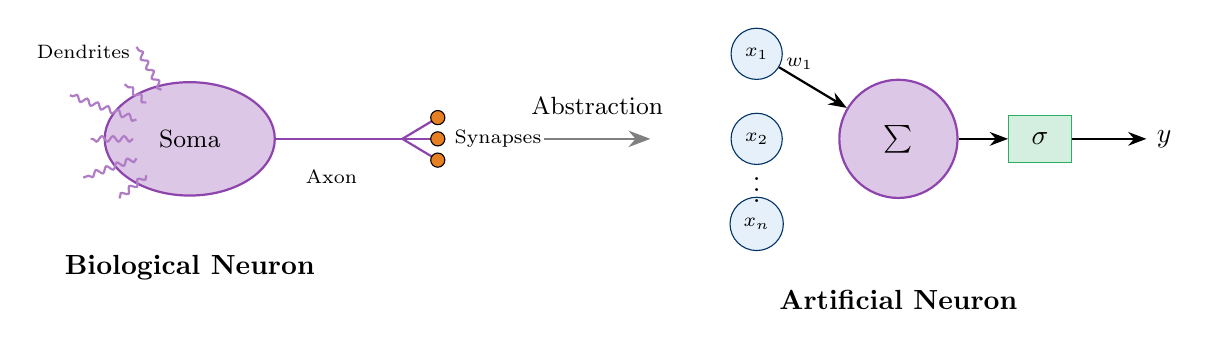
\begin{tikzpicture}[scale=0.9]
    % Biological neuron
    \begin{scope}[shift={(-4,0)}]
        % Cell body
        \draw[fill=neuronpurple!30, draw=neuronpurple, thick] (0,0) ellipse (1.2 and 0.8);
        \node at (0,0) {\small Soma};

        % Dendrites
        \foreach \angle/\len in {120/1.5, 140/1.2, 160/1.8, 180/1.4, 200/1.6, 220/1.3} {
            \draw[thick, neuronpurple!70, decorate, decoration={snake, amplitude=1pt, segment length=4pt}]
                ({\angle}:0.8) -- ({\angle}:\len);
        }

        % Axon
        \draw[thick, neuronpurple] (0:1.2) -- (3,0);

        % Axon terminals
        \foreach \y in {0.3, 0, -0.3} {
            \draw[thick, neuronpurple] (3,0) -- (3.5,\y);
            \draw[fill=accentorange] (3.5,\y) circle (0.1);
        }

        \node[below] at (0,-1.5) {\textbf{Biological Neuron}};
        \node[above, font=\scriptsize] at (-1.5,1) {Dendrites};
        \node[below, font=\scriptsize] at (2,-0.3) {Axon};
        \node[right, font=\scriptsize] at (3.6,0) {Synapses};
    \end{scope}

    % Arrow
    \draw[-{Stealth[scale=1.2]}, thick, gray] (1,0) -- (2.5,0);
    \node[above, font=\small] at (1.75,0.2) {Abstraction};

    % Artificial neuron
    \begin{scope}[shift={(6,0)}]
        % Input nodes
        \node[circle, draw=darkblue, fill=lightblue, minimum size=0.6cm] (inA) at (-2,1.2) {\scriptsize$x_1$};
        \node[circle, draw=darkblue, fill=lightblue, minimum size=0.6cm] (inB) at (-2,0) {\scriptsize$x_2$};
        \node[circle, draw=darkblue, fill=lightblue, minimum size=0.6cm] (inC) at (-2,-1.2) {\scriptsize$x_n$};
        \node at (-2, -0.6) {$\vdots$};

        % Neuron body
        \node[circle, draw=neuronpurple, fill=neuronpurple!30, minimum size=1.5cm, thick] (neuron) at (0,0) {$\sum$};

        % Weights - position labels near the input nodes to avoid overlap
        \draw[-{Stealth}, thick] (inA) -- (neuron) node[pos=0.3, above, font=\scriptsize] {$w_1$};

        % Activation
        \node[rectangle, draw=spikegreen, fill=spikegreen!20, minimum width=0.8cm, minimum height=0.6cm] (act) at (2,0) {$\sigma$};
        \draw[-{Stealth}, thick] (neuron) -- (act);

        % Output
        \draw[-{Stealth}, thick] (act) -- (3.5,0) node[right] {$y$};

        \node[below] at (0,-2) {\textbf{Artificial Neuron}};
    \end{scope}
\end{tikzpicture}
\caption{From biology to mathematics: a biological neuron and its artificial counterpart.}
\label{fig:neuron-comparison}
\end{figure}

\subsection{Artificial Neural Networks}

An artificial neural network takes this biological metaphor and turns it into mathematics. Each artificial neuron:

\begin{enumerate}
    \item Receives inputs from other neurons (or from external data)
    \item Multiplies each input by a \textbf{weight} (representing synaptic strength)
    \item Sums all the weighted inputs
    \item Applies an \textbf{activation function} to produce an output
\end{enumerate}

Mathematically, a single neuron computes:
\begin{equation}
    y = \sigma\left(\sum_{i=1}^{n} w_i x_i + b\right)
\end{equation}

where $x_i$ are inputs, $w_i$ are weights, $b$ is a bias term, and $\sigma$ is the activation function.

\begin{tcolorbox}[keypoint]
\textbf{Key Difference:} Biological neurons communicate through discrete \textit{spikes}, brief electrical pulses. Traditional artificial neural networks (ANNs) use continuous values instead. This distinction becomes important when we discuss spiking neural networks later.
\end{tcolorbox}

\subsection{Brain vs. Artificial Networks: A Comparison}

\begin{table}[H]
\centering
\begin{tabular}{lll}
\toprule
\textbf{Aspect} & \textbf{Brain} & \textbf{Modern LLMs} \\
\midrule
Number of neurons/parameters & $\sim$86 billion & 1--2+ trillion \\
Connections per neuron & $\sim$7,000 & Varies (attention spans all tokens) \\
Communication & Discrete spikes & Continuous values \\
Processing & Massively parallel & Parallel (GPU clusters) \\
Power consumption & $\sim$20 watts & 100s of kW (inference clusters) \\
Precision & Noisy, variable & 16/32-bit floating point \\
Learning & Continuous, local & Batched, global (backprop) \\
\bottomrule
\end{tabular}
\caption{Comparison between biological and modern artificial neural networks.}
\end{table}

The brain's energy efficiency is striking: it performs complex cognition on roughly the power of a dim light bulb. This is a key motivation for neuromorphic computing.

% ============================================
\section{ANNs vs SNNs: Two Paradigms}
% ============================================

There are two different approaches to neural computation: Artificial Neural Networks (ANNs) and Spiking Neural Networks (SNNs). Understanding the distinction matters for this project.

\subsection{Artificial Neural Networks (ANNs)}

ANNs, the workhorses of modern deep learning, process information in discrete layers. Information flows forward through the network, with each layer transforming its inputs through weighted sums and activation functions. The key characteristic: neurons output \textit{continuous values}.

\begin{figure}[H]
\centering
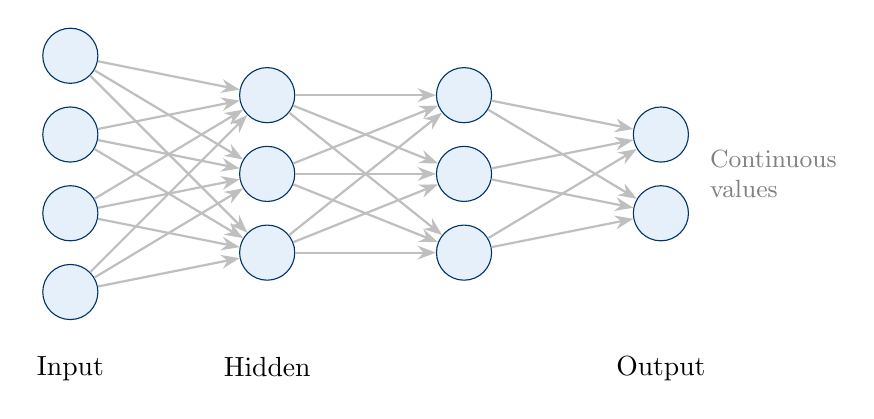
\begin{tikzpicture}[
    neuron/.style={circle, draw=darkblue, fill=lightblue, minimum size=0.7cm},
    arrow/.style={-{Stealth}, thick}
]
    % Input layer
    \node[neuron] (i1) at (0, 1.5) {};
    \node[neuron] (i2) at (0, 0.5) {};
    \node[neuron] (i3) at (0, -0.5) {};
    \node[neuron] (i4) at (0, -1.5) {};
    \node[below] at (0, -2.2) {Input};

    % Hidden layer 1
    \node[neuron] (h1a) at (2.5, 1) {};
    \node[neuron] (h1b) at (2.5, 0) {};
    \node[neuron] (h1c) at (2.5, -1) {};
    \node[below] at (2.5, -2.2) {Hidden};

    % Hidden layer 2
    \node[neuron] (h2a) at (5, 1) {};
    \node[neuron] (h2b) at (5, 0) {};
    \node[neuron] (h2c) at (5, -1) {};

    % Output
    \node[neuron] (o1) at (7.5, 0.5) {};
    \node[neuron] (o2) at (7.5, -0.5) {};
    \node[below] at (7.5, -2.2) {Output};

    % Connections - Input to Hidden 1
    \foreach \i in {i1, i2, i3, i4} {
        \foreach \h in {h1a, h1b, h1c} {
            \draw[arrow, gray!50] (\i) -- (\h);
        }
    }
    % Hidden 1 to Hidden 2
    \foreach \i in {h1a, h1b, h1c} {
        \foreach \h in {h2a, h2b, h2c} {
            \draw[arrow, gray!50] (\i) -- (\h);
        }
    }
    % Hidden 2 to Output
    \foreach \i in {h2a, h2b, h2c} {
        \foreach \h in {o1, o2} {
            \draw[arrow, gray!50] (\i) -- (\h);
        }
    }

    % Values annotation
    \node[right, font=\small, text=gray, align=left] at (8, 0) {Continuous\\values};
\end{tikzpicture}
\caption{A feedforward ANN: information flows from input to output through hidden layers.}
\end{figure}

\subsection{Spiking Neural Networks (SNNs)}

SNNs take a different approach. Rather than passing continuous values, neurons communicate through \textit{spikes}: discrete, all-or-nothing events. This mirrors biological neurons more closely, but introduces a new dimension: \textbf{time}.

In an SNN:
\begin{itemize}
    \item Neurons maintain an internal state (membrane potential)
    \item Incoming spikes cause this potential to rise
    \item When potential crosses a threshold, the neuron fires its own spike
    \item After firing, the potential resets
\end{itemize}

\begin{figure}[H]
\centering

\includegraphics[width=0.95\textwidth]{../gilgamesh/neuron_comparison/comparison.png}
\caption{Gilgamesh vs ngspice validation: membrane potential traces (top), pulse outputs (middle), and error analysis (bottom). Both simulators produce 34 matching spikes, validating our physics model.}
\end{figure}

\subsection{Key Differences}

\begin{table}[H]
\centering
\begin{tabular}{lll}
\toprule
\textbf{Aspect} & \textbf{ANN} & \textbf{SNN} \\
\midrule
Communication & Continuous values & Binary spikes \\
Temporal dynamics & None (static) & Explicit time dimension \\
Computation & Multiply-accumulate & Event-driven \\
Training & Backpropagation (easy) & More challenging \\
Hardware efficiency & Power-hungry & Potentially very efficient \\
Biological realism & Low & Higher \\
\bottomrule
\end{tabular}
\end{table}

\begin{tcolorbox}[keypoint]
\textbf{Why SNNs for hardware?} The event-driven nature of SNNs means computation only happens when spikes occur. In sparse networks, this can reduce energy consumption by orders of magnitude: a neuron that isn't spiking consumes almost no power.
\end{tcolorbox}

% ============================================
\section{The Leaky Integrate-and-Fire Neuron}
% ============================================

The Leaky Integrate-and-Fire (LIF) neuron is the workhorse of computational neuroscience and neuromorphic engineering. It captures the core dynamics of biological neurons while remaining simple enough to simulate efficiently and implement in hardware.

\subsection{The Model}

The LIF neuron treats the cell membrane as a leaky capacitor. Input current charges the membrane, but charge also leaks away over time. The dynamics are governed by:

\begin{equation}
    \tau_m \frac{dV}{dt} = -V + R \cdot I(t)
\end{equation}

where:
\begin{itemize}
    \item $V$ is the membrane potential
    \item $\tau_m = RC$ is the membrane time constant
    \item $R$ is the membrane resistance
    \item $I(t)$ is the input current
\end{itemize}

When $V$ crosses a threshold $\theta$, the neuron emits a spike and resets.

\subsection{Circuit Analogy}

The LIF neuron has a direct circuit interpretation, which makes it well-suited for hardware implementation:

\begin{figure}[H]
\centering
\includegraphics[width=0.6\textwidth]{../lifcircuit.png}
\caption{Our LIF neuron circuit implementation. The RC network ($R_L$, $C_M$) integrates synaptic current while providing natural leakage. The op-amp buffer isolates the membrane voltage, and the comparator detects threshold crossings to generate spikes.}
\label{fig:lif-circuit}
\end{figure}

\subsection{Discrete-Time Implementation}

For simulation and training, we discretise the continuous dynamics. With timestep $\Delta t$:

\begin{equation}
    V[t+1] = \beta \cdot V[t] + I[t]
\end{equation}

where $\beta = e^{-\Delta t / \tau_m}$ is the decay factor (typically $\sim$0.9).

The spike generation and reset:
\begin{align}
    S[t] &= \mathcal{H}(V[t] - \theta) \\
    V_{reset}[t] &= V[t] - \theta \cdot S[t]
\end{align}

where $\mathcal{H}$ is the Heaviside step function.

\begin{tcolorbox}[infobox]
\textbf{Typical Parameters:}
\begin{itemize}
    \item Membrane time constant: $\tau_m \approx 4$--$10$ ms
    \item Threshold: $\theta = 1.0$ (normalised)
    \item Decay factor: $\beta = 0.9$
    \item In our hardware: $R = 120\,\text{k}\Omega$, $C = 33\,\text{nF}$, giving $\tau_m \approx 4\,\text{ms}$
\end{itemize}
\end{tcolorbox}

% ============================================
\section{ngspice: Circuit Simulation}
% ============================================

\textbf{ngspice} is an open-source circuit simulator, the modern descendant of SPICE (Simulation Program with Integrated Circuit Emphasis), originally developed at Berkeley in the 1970s. It has become the industry standard for analog and mixed-signal circuit simulation.

\subsection{Why ngspice?}

For neuromorphic hardware development, ngspice serves a critical role: it lets us verify that our abstract neuron models match the behaviour of real transistor-level circuits.

\begin{figure}[H]
\centering
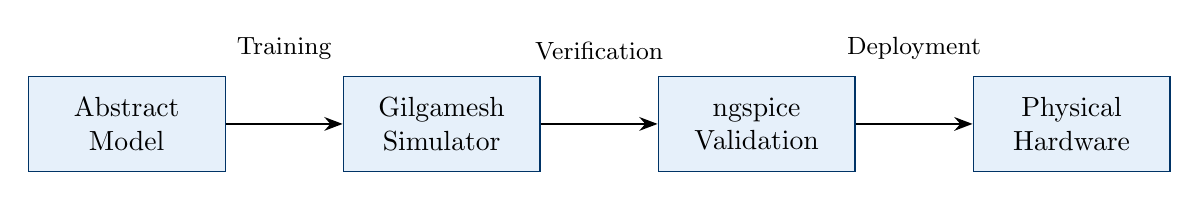
\begin{tikzpicture}[
    box/.style={rectangle, draw=darkblue, fill=lightblue, minimum width=2.5cm, minimum height=1.2cm, align=center},
    arrow/.style={-{Stealth}, thick}
]
    \node[box] (model) at (0,0) {Abstract\\Model};
    \node[box] (sim) at (4,0) {Gilgamesh\\Simulator};
    \node[box] (spice) at (8,0) {ngspice\\Validation};
    \node[box] (hw) at (12,0) {Physical\\Hardware};

    \draw[arrow] (model) -- (sim);
    \draw[arrow] (sim) -- (spice);
    \draw[arrow] (spice) -- (hw);

    \node[above, font=\small] at (2,0.7) {Training};
    \node[above, font=\small] at (6,0.7) {Verification};
    \node[above, font=\small] at (10,0.7) {Deployment};
\end{tikzpicture}
\caption{The development pipeline: from abstract models to verified hardware.}
\end{figure}

\subsection{What ngspice Does}

ngspice solves the differential equations that govern electronic circuits:
\begin{itemize}
    \item \textbf{Transient analysis:} Simulates circuit behaviour over time
    \item \textbf{DC analysis:} Finds steady-state operating points
    \item \textbf{AC analysis:} Analyses frequency response
    \item \textbf{Monte Carlo:} Models component variations and manufacturing tolerances
\end{itemize}

For our neurons, ngspice can simulate the exact voltage waveforms, accounting for:
\begin{itemize}
    \item Parasitic capacitances and resistances
    \item Transistor non-idealities
    \item Temperature variations
    \item Component tolerances
\end{itemize}

\subsection{Gilgamesh-ngspice Integration}

We use ngspice to verify that Gilgamesh's physics models accurately match transistor-level circuit behaviour. This validation process involves:
\begin{enumerate}
    \item Simulating individual LIF neurons in both Gilgamesh and ngspice
    \item Comparing membrane voltage traces and spike timing
    \item Measuring error metrics (RMS error, correlation)
    \item Iterating on Gilgamesh's physics parameters until they match
\end{enumerate}

This ensures that when we move to hardware, the behaviour we trained for in simulation will actually occur in the physical circuit.

% ============================================
\section{Rust: The Implementation Language}
% ============================================

Gilgamesh is written in \textbf{Rust}, a systems programming language increasingly used for performance-critical applications. But why Rust for a neural network simulator?

\subsection{Key Features}

\begin{description}
    \item[Memory safety without garbage collection:] Rust's ownership system prevents entire classes of bugs (null pointer dereferences, buffer overflows, data races) at compile time. This matters when simulating thousands of neurons over millions of timesteps.

    \item[Zero-cost abstractions:] High-level code compiles to efficient machine code. We can write expressive, maintainable code without sacrificing performance.

    \item[Fearless concurrency:] Rust's type system prevents data races, making it safe to parallelise across neurons and timesteps.

    \item[C/C++ interoperability:] We can call existing libraries (like BLAS for linear algebra) when needed.
\end{description}

\subsection{Performance Comparison}

\begin{table}[H]
\centering
\begin{tabular}{lccc}
\toprule
\textbf{Language} & \textbf{Speed} & \textbf{Memory Safety} & \textbf{Ease of Use} \\
\midrule
C/C++ & Excellent & Manual & Moderate \\
Python & Poor & Automatic & Excellent \\
Rust & Excellent & Automatic & Moderate \\
\bottomrule
\end{tabular}
\caption{Rust offers the performance of C with the safety of managed languages.}
\end{table}

\subsection{Example: LIF Forward Pass}

Here's a taste of how Gilgamesh implements the LIF forward pass in Rust:

\begin{lstlisting}[language=Rust, caption={Simplified LIF forward pass in Rust}]
fn forward(&self, input: &Array1<f32>, mem: &mut Array1<f32>)
    -> Array1<f32> {
    // Update membrane potential
    *mem = &*mem * self.beta + input;

    // Generate spikes where threshold exceeded
    let spikes = mem.mapv(|v| if v > self.threshold { 1.0 } else { 0.0 });

    // Reset spiked neurons
    *mem = mem - &spikes * self.threshold;

    spikes
}
\end{lstlisting}

The code is concise, readable, and compiles to highly optimised machine code.

% ============================================
\section{Gilgamesh: Our SNN Simulator}
% ============================================

\textbf{Gilgamesh} is a hardware-accurate spiking neural network simulator developed as part of the Tarskii project. Named after the ancient Mesopotamian king, Gilgamesh bridges the gap between abstract neural network models and physical neuromorphic hardware.

\subsection{Design Philosophy}

Gilgamesh operates in two modes:

\begin{description}
    \item[Simple Mode:] Fast simulation compatible with frameworks like snnTorch. Uses discrete-time dynamics with a decay factor $\beta$. Good for rapid prototyping and training.

    \item[Physics Mode:] Accurate RC-circuit dynamics matching real hardware. Uses physical parameters (resistance, capacitance, voltage rails). Required for hardware validation.
\end{description}

\begin{figure}[H]
\centering
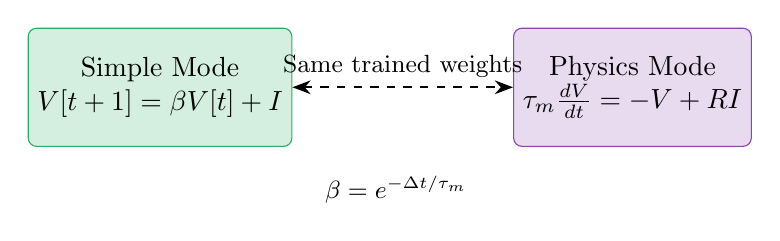
\begin{tikzpicture}[
    box/.style={rectangle, draw, minimum width=3cm, minimum height=1.5cm, align=center, rounded corners=3pt},
    simple/.style={box, draw=spikegreen, fill=spikegreen!20},
    physics/.style={box, draw=neuronpurple, fill=neuronpurple!20}
]
    \node[simple] (s1) at (0,0) {Simple Mode\\$V[t+1] = \beta V[t] + I$};
    \node[physics] (p1) at (6,0) {Physics Mode\\$\tau_m \frac{dV}{dt} = -V + RI$};

    \draw[{Stealth}-{Stealth}, thick, dashed] (s1) -- (p1)
        node[midway, above, font=\small] {Same trained weights};
    \node[below, font=\small] at (3,-1) {$\beta = e^{-\Delta t/\tau_m}$};
\end{tikzpicture}
\caption{Gilgamesh's dual-mode architecture: train fast, validate accurately.}
\end{figure}

\subsection{Network Architecture}

Our hardware-optimised network for MNIST classification uses a compact 36-12-10 architecture:

\begin{figure}[H]
\centering
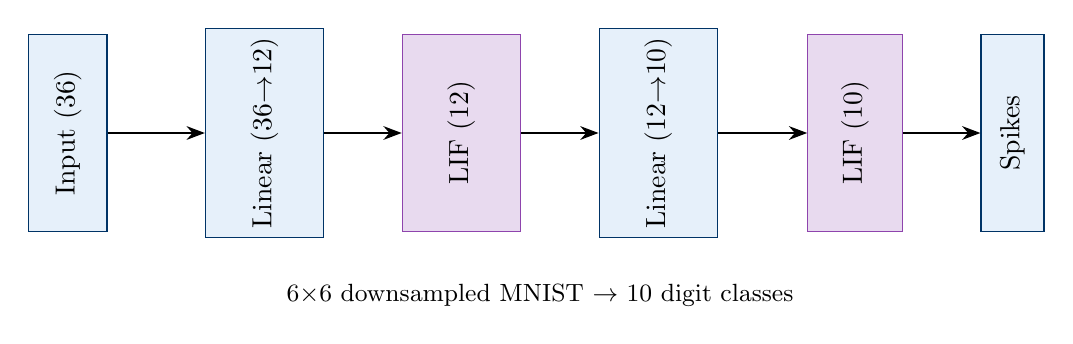
\begin{tikzpicture}[
    layer/.style={rectangle, draw=darkblue, fill=lightblue, minimum height=2.5cm, align=center},
    arrow/.style={-{Stealth}, thick}
]
    % Input
    \node[layer, minimum width=1cm] (input) at (0,0) {\rotatebox{90}{Input (36)}};

    % FC1
    \node[layer, minimum width=1.5cm] (fc1) at (2.5,0) {\rotatebox{90}{Linear (36$\to$12)}};

    % LIF1
    \node[layer, minimum width=1.5cm, draw=neuronpurple, fill=neuronpurple!20] (lif1) at (5,0) {\rotatebox{90}{LIF (12)}};

    % FC2
    \node[layer, minimum width=1.5cm] (fc2) at (7.5,0) {\rotatebox{90}{Linear (12$\to$10)}};

    % LIF2
    \node[layer, minimum width=1.2cm, draw=neuronpurple, fill=neuronpurple!20] (lif2) at (10,0) {\rotatebox{90}{LIF (10)}};

    % Output
    \node[layer, minimum width=0.8cm] (output) at (12,0) {\rotatebox{90}{Spikes}};

    \draw[arrow] (input) -- (fc1);
    \draw[arrow] (fc1) -- (lif1);
    \draw[arrow] (lif1) -- (fc2);
    \draw[arrow] (fc2) -- (lif2);
    \draw[arrow] (lif2) -- (output);

    \node[below, font=\small] at (6,-1.8) {6$\times$6 downsampled MNIST $\to$ 10 digit classes};
\end{tikzpicture}
\caption{Gilgamesh network architecture. LIF neurons are shown in purple.}
\end{figure}

\textbf{Total synapses:} 552 (36$\times$12 + 12$\times$10)

\textbf{Achieved accuracy:} 90.69\% on MNIST test set

This architecture was chosen through iterative search, balancing accuracy against hardware complexity. Beyond 90\% accuracy, the additional synapses required yield diminishing returns for our target applications.

\subsection{Key Features}

\begin{itemize}
    \item \textbf{Hardware parameter mapping:} Converts normalised weights to physical currents and voltages
    \item \textbf{SPICE validation:} Generate ngspice simulations to verify physics models
    \item \textbf{Multiple surrogate gradients:} FastSigmoid, ATan, Sigmoid, Straight-Through
    \item \textbf{Physics effects:} Pulse stretching, threshold adaptation, comparator delays
    \item \textbf{Quantisation support:} 4-bit weights for current source DAC implementation
    \item \textbf{Visualisation:} Real-time dashboards for spike activity
\end{itemize}

% ============================================
\section{The Mathematics of Gilgamesh}
% ============================================

This section details the mathematical foundations underpinning Gilgamesh.

\subsection{LIF Dynamics}

\subsubsection{Simple Mode}
\begin{align}
    V[t+1] &= \beta \cdot V[t] + I[t] \\
    S[t] &= \mathcal{H}(V[t] - \theta) \\
    V_{reset}[t] &= V[t+1] - \theta \cdot S[t]
\end{align}

\subsubsection{Physics Mode}
\begin{align}
    \frac{dV}{dt} &= \frac{I_{syn}}{C} - \frac{V}{\tau_m} \\
    \text{Discretised:} \quad V[t+1] &= I \cdot \tau_m \cdot (1 - e^{-\Delta t/\tau_m}) + V[t] \cdot e^{-\Delta t/\tau_m}
\end{align}

The connection: $\beta = e^{-\Delta t/\tau_m}$, so physics mode reduces to simple mode when appropriately parameterised.

\subsection{Spike Generation}

The spike function is a Heaviside step:
\begin{equation}
    S = \mathcal{H}(V - \theta) = \begin{cases} 1 & \text{if } V > \theta \\ 0 & \text{otherwise} \end{cases}
\end{equation}

\subsection{Loss Function}

Classification uses cross-entropy on spike counts:
\begin{align}
    c_i &= \sum_{t=1}^{T} S_i[t] \quad \text{(spike count for class } i\text{)} \\
    p_i &= \frac{e^{c_i}}{\sum_j e^{c_j}} \quad \text{(softmax)} \\
    \mathcal{L} &= -\log(p_{target})
\end{align}

\subsection{Optimisation}

Gilgamesh uses Adam with weight decay (AdamW):
\begin{align}
    m_t &= \beta_1 m_{t-1} + (1-\beta_1) \nabla \mathcal{L} \\
    v_t &= \beta_2 v_{t-1} + (1-\beta_2) (\nabla \mathcal{L})^2 \\
    \hat{m}_t &= \frac{m_t}{1-\beta_1^t}, \quad \hat{v}_t = \frac{v_t}{1-\beta_2^t} \\
    w_{t+1} &= w_t - \eta \left( \frac{\hat{m}_t}{\sqrt{\hat{v}_t} + \epsilon} + \lambda w_t \right)
\end{align}

Default parameters: $\eta = 0.001$, $\beta_1 = 0.9$, $\beta_2 = 0.999$, $\epsilon = 10^{-8}$, $\lambda = 0.01$

% ============================================
\section{Backpropagation and BPTT}
% ============================================

Training neural networks requires computing how to adjust weights to reduce errors. This is done through \textbf{backpropagation}: propagating error signals backwards through the network.

\subsection{Standard Backpropagation}

For a feedforward network, backpropagation applies the chain rule layer by layer:

\begin{equation}
    \frac{\partial \mathcal{L}}{\partial w_i} = \frac{\partial \mathcal{L}}{\partial y} \cdot \frac{\partial y}{\partial z} \cdot \frac{\partial z}{\partial w_i}
\end{equation}

where $z$ is the pre-activation and $y$ is the output.

\begin{figure}[H]
\centering
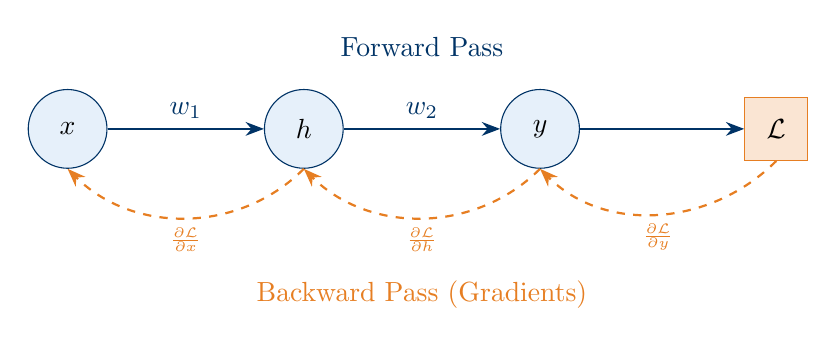
\begin{tikzpicture}[
    node/.style={circle, draw=darkblue, fill=lightblue, minimum size=1cm},
    arrow/.style={-{Stealth}, thick}
]
    % Forward pass
    \node[node] (x) at (0,0) {$x$};
    \node[node] (h) at (3,0) {$h$};
    \node[node] (y) at (6,0) {$y$};
    \node[rectangle, draw=accentorange, fill=accentorange!20, minimum size=0.8cm] (L) at (9,0) {$\mathcal{L}$};

    \draw[arrow, darkblue] (x) -- (h) node[midway, above] {$w_1$};
    \draw[arrow, darkblue] (h) -- (y) node[midway, above] {$w_2$};
    \draw[arrow, darkblue] (y) -- (L);

    % Backward pass (below the nodes)
    \draw[arrow, accentorange, dashed] (L.south) to[out=-135,in=-45] node[midway, below, font=\scriptsize] {$\frac{\partial \mathcal{L}}{\partial y}$} (y.south);
    \draw[arrow, accentorange, dashed] (y.south) to[out=-135,in=-45] node[midway, below, font=\scriptsize] {$\frac{\partial \mathcal{L}}{\partial h}$} (h.south);
    \draw[arrow, accentorange, dashed] (h.south) to[out=-135,in=-45] node[midway, below, font=\scriptsize] {$\frac{\partial \mathcal{L}}{\partial x}$} (x.south);

    \node[above] at (4.5, 0.8) {\color{darkblue}Forward Pass};
    \node[below] at (4.5, -1.8) {\color{accentorange}Backward Pass (Gradients)};
\end{tikzpicture}
\caption{Backpropagation: gradients flow backward from the loss to update weights.}
\end{figure}

\subsection{Backpropagation Through Time (BPTT)}

SNNs have recurrent dynamics: the membrane potential at time $t$ depends on time $t-1$. This temporal dependency requires \textbf{Backpropagation Through Time} (BPTT).

\begin{figure}[H]
\centering
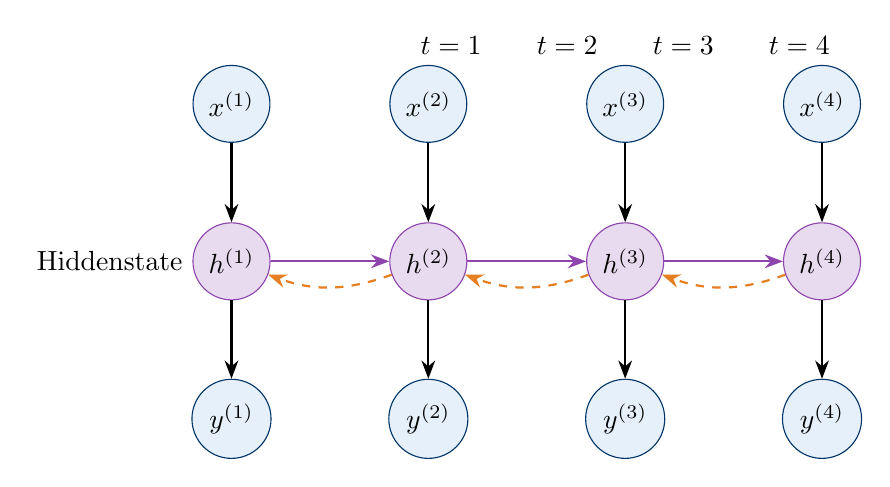
\begin{tikzpicture}[
    node/.style={circle, draw=darkblue, fill=lightblue, minimum size=0.9cm},
    state/.style={circle, draw=neuronpurple, fill=neuronpurple!20, minimum size=0.9cm},
    arrow/.style={-{Stealth}, thick}
]
    % Unrolled timesteps
    \foreach \t in {1,2,3,4} {
        \node[node] (x\t) at (\t*2.5 - 2.5, 2) {$x^{(\t)}$};
        \node[state] (h\t) at (\t*2.5 - 2.5, 0) {$h^{(\t)}$};
        \node[node] (y\t) at (\t*2.5 - 2.5, -2) {$y^{(\t)}$};

        \draw[arrow] (x\t) -- (h\t);
        \draw[arrow] (h\t) -- (y\t);
    }

    % Recurrent connections
    \draw[arrow, neuronpurple] (h1) -- (h2);
    \draw[arrow, neuronpurple] (h2) -- (h3);
    \draw[arrow, neuronpurple] (h3) -- (h4);

    % Labels
    \node[left] at (-0.5, 0) {Hidden\\state};
    \node[above] at (5, 2.5) {$t=1 \quad\quad t=2 \quad\quad t=3 \quad\quad t=4$};

    % BPTT arrows (dashed, going backwards)
    \draw[arrow, accentorange, dashed] (h4) to[bend left=20] (h3);
    \draw[arrow, accentorange, dashed] (h3) to[bend left=20] (h2);
    \draw[arrow, accentorange, dashed] (h2) to[bend left=20] (h1);
\end{tikzpicture}
\caption{BPTT unrolls the network in time. Gradients (orange, dashed) flow backwards through both layers and timesteps.}
\end{figure}

The gradient through the membrane state:
\begin{equation}
    \frac{\partial \mathcal{L}}{\partial V[t]} = \frac{\partial \mathcal{L}}{\partial S[t]} \cdot \frac{\partial S[t]}{\partial V[t]} + \frac{\partial \mathcal{L}}{\partial V[t+1]} \cdot \frac{\partial V[t+1]}{\partial V[t]}
\end{equation}

The second term captures how past membrane states affect future outputs. This is the ``through time'' component.

\begin{tcolorbox}[keypoint]
\textbf{The problem:} $\frac{\partial S}{\partial V} = \frac{d\mathcal{H}}{dV}$ is zero everywhere except at the threshold, where it's undefined. The Heaviside function has no useful gradient for learning!
\end{tcolorbox}

% ============================================
\section{Surrogate Gradients}
% ============================================

The non-differentiability of spike generation is the central challenge of training SNNs. \textbf{Surrogate gradients} provide a practical workaround.

\subsection{The Problem}

The Heaviside step function $\mathcal{H}(x)$ has derivative:
\begin{equation}
    \frac{d\mathcal{H}}{dx} = \begin{cases} 0 & \text{if } x \neq 0 \\ \text{undefined} & \text{if } x = 0 \end{cases}
\end{equation}

With zero gradients, backpropagation cannot update weights. The network cannot learn.

\subsection{The Solution}

Use a smooth, differentiable function as a \textit{surrogate} during the backward pass:
\begin{itemize}
    \item \textbf{Forward pass:} Use the true Heaviside (binary spikes)
    \item \textbf{Backward pass:} Use a smooth approximation (non-zero gradients)
\end{itemize}

\begin{figure}[H]
\centering
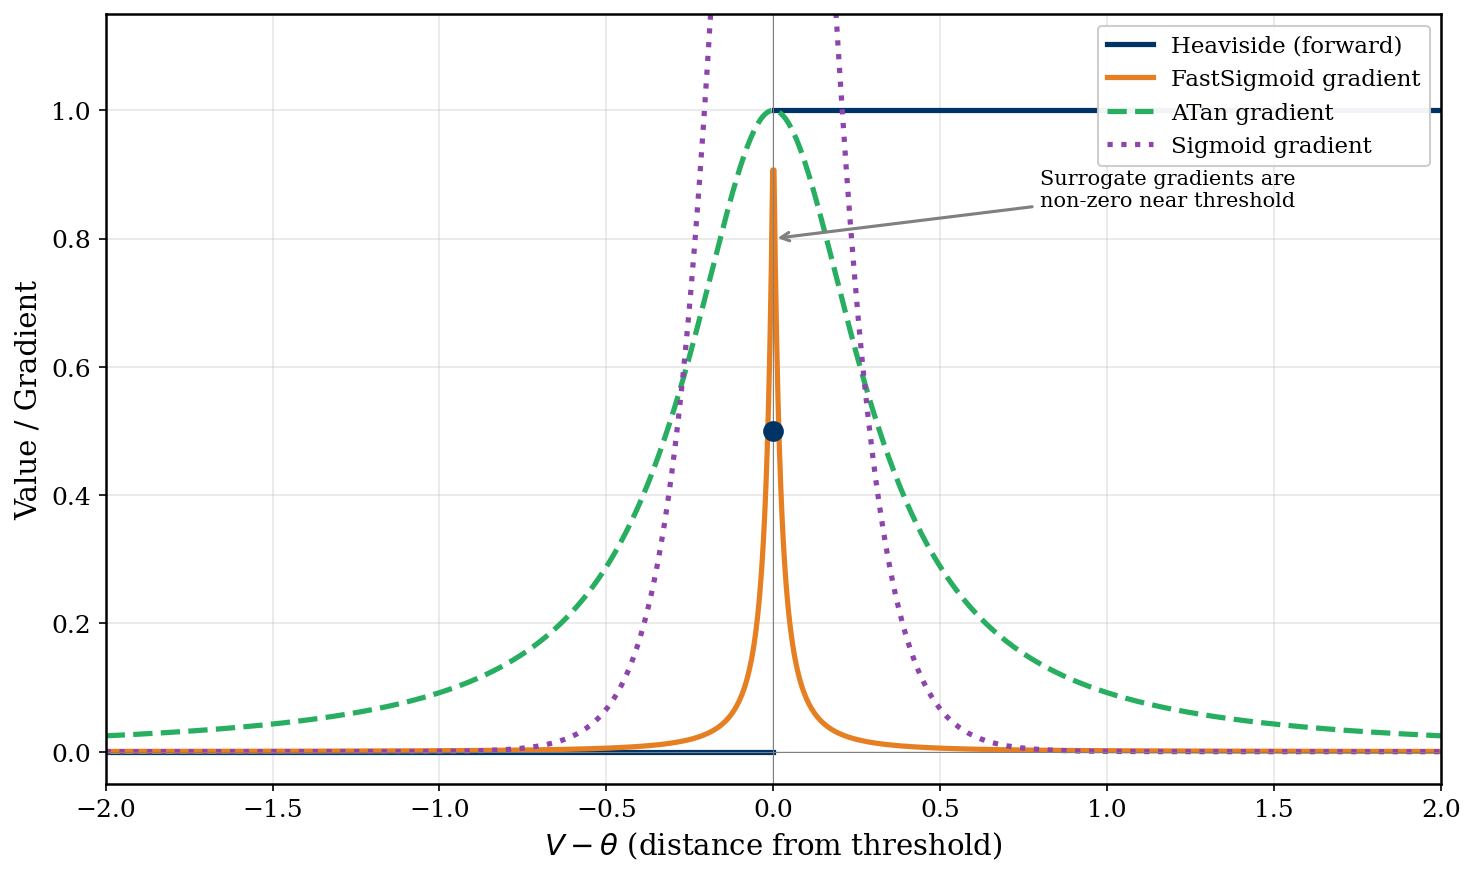
\includegraphics[width=0.85\textwidth]{surrogate_gradients.png}
\caption{Surrogate gradients provide smooth, non-zero derivatives where the Heaviside has none. The peak at $V=\theta$ allows gradients to flow during backpropagation.}
\end{figure}

\subsection{Surrogate Functions in Gilgamesh}

\textbf{FastSigmoid (SuperSpike)}, default, slope $k=25$:
\begin{equation}
    \sigma'(x) \approx \frac{1}{(k|x| + 1)^2}
\end{equation}

\textbf{ATan}, snnTorch default, $\alpha=2$:
\begin{equation}
    \sigma'(x) \approx \frac{\alpha/2}{1 + (\pi \alpha x / 2)^2}
\end{equation}

\textbf{Sigmoid}, classical, slope $k$:
\begin{equation}
    \sigma'(x) \approx \frac{k \cdot e^{-kx}}{(e^{-kx} + 1)^2}
\end{equation}

\textbf{Straight-Through Estimator:}
\begin{equation}
    \sigma'(x) = 1 \quad \text{(everywhere)}
\end{equation}

\begin{tcolorbox}[infobox]
\textbf{Intuition:} Surrogate gradients say ``when the membrane is close to threshold, small changes matter a lot; when it's far from threshold, they don't.'' The slope parameter controls how sharply this transition occurs.
\end{tcolorbox}

% ============================================
\section{Ireland's Data Centre Problem}
% ============================================

Ireland has become a European hub for data centres, hosting facilities for Google, Amazon, Microsoft, Meta, and many others. But this success has created a significant energy challenge.

\subsection{The Scale of the Problem}

\begin{tcolorbox}[keypoint]
\textbf{Key statistic:} Data centres now consume approximately \textbf{21\% of Ireland's total electricity}, more than all urban households combined.
\end{tcolorbox}

\begin{figure}[H]
\centering
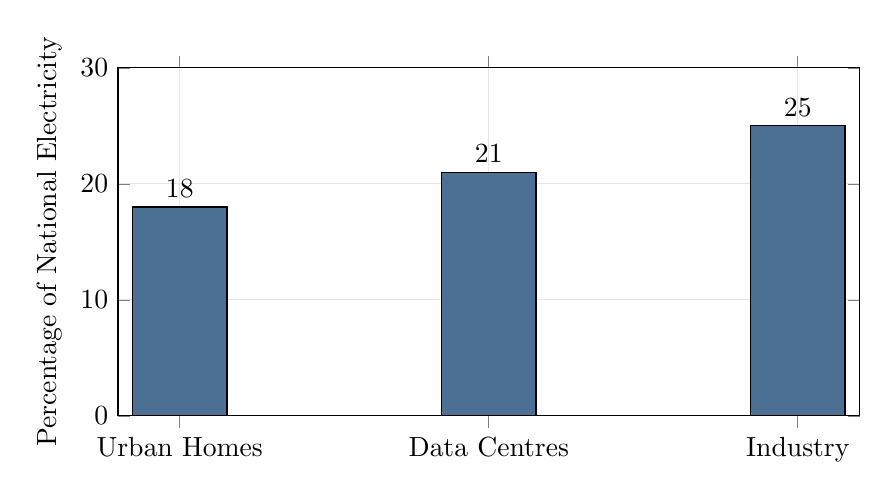
\begin{tikzpicture}
    \begin{axis}[
        width=11cm, height=6cm,
        ybar,
        bar width=1.2cm,
        xlabel={},
        ylabel={Percentage of National Electricity},
        symbolic x coords={Urban Homes, Data Centres, Industry},
        xtick=data,
        ymin=0, ymax=30,
        nodes near coords,
        nodes near coords align={vertical},
        grid=both,
        grid style={gray!20},
    ]
        \addplot[fill=darkblue!70] coordinates {
            (Urban Homes, 18)
            (Data Centres, 21)
            (Industry, 25)
        };
    \end{axis}
\end{tikzpicture}
\caption{Ireland's electricity consumption by sector (approximate, 2024).}
\end{figure}

\subsection{Why Ireland?}

Several factors made Ireland attractive for data centres:
\begin{itemize}
    \item Cool climate (reducing cooling costs)
    \item EU membership and data sovereignty
    \item English-speaking workforce
    \item Favourable corporate tax environment
    \item Strong renewable energy potential
\end{itemize}

\subsection{The Grid Strain}

EirGrid, Ireland's transmission system operator, has raised concerns:
\begin{itemize}
    \item Data centres strain the grid during peak demand
    \item New connections have been restricted in the Dublin region
    \item Renewable energy targets become harder to meet
    \item Industrial users face higher electricity costs
\end{itemize}

\subsection{AI Exacerbates the Problem}

Modern AI workloads are particularly power-hungry:
\begin{itemize}
    \item Training large language models can consume megawatts for weeks
    \item Inference at scale (serving millions of users) requires constant power
    \item GPU clusters generate significant heat, requiring energy-intensive cooling
    \item AI chip manufacturing is itself energy-intensive
\end{itemize}

% ============================================
\section{AI's Energy Challenge}
% ============================================

The explosive growth of AI has brought its energy consumption into sharp focus. While training costs grab headlines, \textbf{inference at scale} is where the real energy crisis lies.

\subsection{The Inference Problem}

Training happens once; inference happens billions of times per day. Consider Google's Gemini:
\begin{itemize}
    \item Over \textbf{650 million monthly active users} as of late 2025
    \item \textbf{35--45 million daily active users} making queries
    \item \textbf{1.5 billion monthly AI Overview interactions} in Google Search alone
    \item Gemini 3 Pro is estimated at \textbf{2+ trillion parameters}, larger than models like Kimi K2 (1T parameters)
\end{itemize}

Each query to a model of this scale requires substantial computation, running on hardware like NVIDIA's H200 GPUs.

\subsubsection{Napkin Maths: The Power Bill}

Let's estimate the power consumption for AI inference at scale:

\begin{tcolorbox}[infobox]
\textbf{Assumptions (conservative):}
\begin{itemize}
    \item 40 million daily active users $\times$ 10 queries/day = \textbf{400 million queries/day}
    \item Average $\approx$ 4,600 queries/second, peak $\approx$ 15,000 queries/second
    \item A 2T parameter model needs $\sim$8 H200 GPUs per inference server
    \item Each server handles $\sim$10 queries/second
\end{itemize}
\end{tcolorbox}

\textbf{Working through the numbers:}
\begin{align*}
    \text{Servers needed (peak)} &= \frac{15,000 \text{ queries/s}}{10 \text{ queries/s/server}} = 1,500 \text{ servers} \\[0.5em]
    \text{GPUs} &= 1,500 \times 8 = 12,000 \text{ H200s} \\[0.5em]
    \text{GPU power} &= 12,000 \times 700\text{W} = 8.4 \text{ MW} \\[0.5em]
    \text{With cooling \& infrastructure} &\approx 8.4 \times 2 = \mathbf{17 \text{ MW}}
\end{align*}

Running 24/7/365:
\[
    17 \text{ MW} \times 8,760 \text{ hours} = \mathbf{149 \text{ GWh/year}}
\]

That's just \textit{one} AI service from \textit{one} company. Add tooling, Microsoft, tooling, Meta, and dozens of others, each with millions of users. A reasonable estimate for global AI inference might be \textbf{500+ GWh/year} and climbing.

For context: Ireland's total electricity consumption is roughly 30,000 GWh/year. AI inference alone could soon rival a small country's entire grid demand.

\subsection{The Hardware Reality}

A single NVIDIA H200 GPU consumes \textbf{700 watts} at full load. To serve a model like Gemini 3 Pro to millions of concurrent users requires thousands of these GPUs running continuously. A typical DGX H200 system (8 GPUs) draws over \textbf{10 kilowatts}, enough to power several homes.

\begin{table}[H]
\centering
\begin{tabular}{lccc}
\toprule
\textbf{System} & \textbf{Power} & \textbf{Capability} & \textbf{Speed} \\
\midrule
Human brain & $\sim$20 W & General intelligence & Real-time \\
NVIDIA H200 GPU & $\sim$700 W & Trillion-param LLMs & ms/token \\
DGX H200 (8 GPU) & $\sim$10 kW & Full model inference & ms/token \\
Arduino Nano & $\sim$100 mW & Small SNNs (same as ours) & $\sim$100 ms \\
\textbf{Our SNN chip} & $\sim$\textbf{1 mW} & \textbf{Small SNNs} & \textbf{5 ms} \\
\bottomrule
\end{tabular}
\caption{Power consumption across computing paradigms. An Arduino Nano \textit{can} run the same 552-synapse network as our chip, but at 100$\times$ the power and 20$\times$ slower.}
\end{table}

\begin{tcolorbox}[infobox]
\textbf{Why not just use an Arduino?} You could implement our SNN on a microcontroller. The maths is simple enough. But digital computation burns power on every operation: fetching instructions, moving data, clocking flip-flops. Our analog chip computes through physics itself, consuming energy only when spikes occur. For always-on, battery-powered applications, this difference matters.

\textbf{Looking ahead:} This first-generation chip targets a modest 552-synapse network. Future iterations will scale to larger networks, enabling more complex tasks while maintaining the fundamental efficiency advantage of analog neuromorphic computing.
\end{tcolorbox}

\subsection{The Efficiency Gap}

The brain achieves general intelligence on 20 watts. Modern AI requires megawatts to approximate narrow aspects of that intelligence. This gap exists because conventional computing architectures waste energy shuffling data between memory and processors, the so-called \textbf{von Neumann bottleneck}.

\subsection{Compute-in-Memory: The Holy Grail}

\begin{tcolorbox}[keypoint]
\textbf{The holy grail of edge AI} is a chip that offers high efficiency, performance, and versatility simultaneously. Compute-in-memory architectures promise exactly this by eliminating data movement entirely.
\end{tcolorbox}

In conventional processors, data must travel between separate memory and processing units, consuming energy and time. \textbf{Compute-in-memory} (also called \textit{in-memory computing} or \textit{processing-in-memory}) performs calculations directly where data is stored.

Our analog SNN chip embodies this principle:
\begin{itemize}
    \item \textbf{Weights are stored as physical properties:} resistances or current source settings
    \item \textbf{Computation happens through physics:} Kirchhoff's laws sum currents automatically
    \item \textbf{No data movement required:} inputs flow through the weight matrix in a single pass
    \item \textbf{Massive parallelism:} all synapses compute simultaneously
\end{itemize}

This approach has been called the ``holy grail'' of semiconductor design because it sidesteps the limitations of von Neumann architectures. Major chip manufacturers are pursuing similar ideas, and analog neuromorphic implementations offer strong efficiency gains.

% ============================================
\section{Edge AI and Neuromorphic Solutions}
% ============================================

Moving AI computation from data centres to edge devices (smartphones, sensors, embedded systems) offers clear benefits, but poses challenges that neuromorphic computing may help solve.

\subsection{The Edge Computing Promise}

Running AI at the edge means:
\begin{itemize}
    \item \textbf{Lower latency:} No round-trip to the cloud
    \item \textbf{Privacy:} Data stays on-device
    \item \textbf{Reliability:} Works without internet connectivity
    \item \textbf{Reduced bandwidth:} Only results, not raw data, need transmission
\end{itemize}

\subsection{The Power Wall}

Edge devices face strict power constraints:
\begin{itemize}
    \item Smartphones: $\sim$5 W total budget, AI must share with display, radio, etc.
    \item Wearables: $\sim$100 mW or less
    \item IoT sensors: Often $<$10 mW, potentially harvested from environment
    \item Drones/robots: Battery life directly limits mission duration
\end{itemize}

Running conventional neural networks under these constraints requires either:
\begin{enumerate}
    \item Smaller, less capable models
    \item Aggressive quantisation (reduced precision)
    \item Sparse activation patterns
    \item Specialised accelerators
\end{enumerate}

\subsection{The Neuromorphic Advantage}

Spiking neural networks on analog hardware offer a fundamentally different approach:

\begin{tcolorbox}[keypoint]
\textbf{Event-driven computation:} Unlike conventional chips that compute continuously, neuromorphic hardware only consumes energy when spikes occur. For sparse, real-world signals, this can reduce power by orders of magnitude.
\end{tcolorbox}

\subsubsection{Why Analog?}

\begin{itemize}
    \item \textbf{Physics does the maths:} Currents naturally sum (Kirchhoff's law), capacitors naturally integrate, resistors naturally leak. The differential equations of neural dynamics are solved by physics, not software.

    \item \textbf{No digital overhead:} No clock distribution, no synchronisation, no memory access bottlenecks.

    \item \textbf{Inherent parallelism:} Every neuron computes simultaneously, limited only by physical layout.

    \item \textbf{Low voltage operation:} Analog circuits can operate at lower voltages than digital logic, reducing power quadratically.
\end{itemize}

\subsection{The Tarskii Vision}

Our analog SNN chip aims to enable:

\begin{figure}[H]
\centering
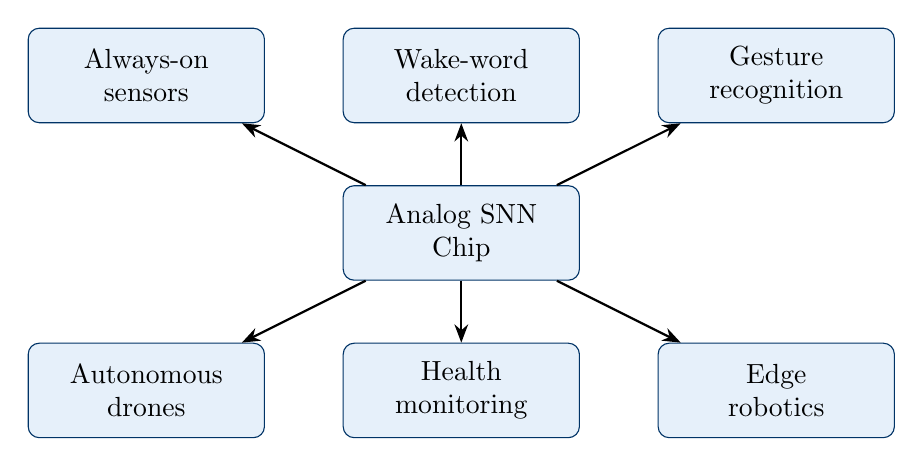
\begin{tikzpicture}[
    app/.style={rectangle, draw=darkblue, fill=lightblue, minimum width=3cm, minimum height=1.2cm, align=center, rounded corners},
    arrow/.style={-{Stealth}, thick}
]
    \node[app] (chip) at (0,0) {Analog SNN\\Chip};

    \node[app] (sensor) at (-4, 2) {Always-on\\sensors};
    \node[app] (wake) at (0, 2) {Wake-word\\detection};
    \node[app] (gesture) at (4, 2) {Gesture\\recognition};

    \node[app] (drone) at (-4, -2) {Autonomous\\drones};
    \node[app] (health) at (0, -2) {Health\\monitoring};
    \node[app] (robot) at (4, -2) {Edge\\robotics};

    \draw[arrow] (chip) -- (sensor);
    \draw[arrow] (chip) -- (wake);
    \draw[arrow] (chip) -- (gesture);
    \draw[arrow] (chip) -- (drone);
    \draw[arrow] (chip) -- (health);
    \draw[arrow] (chip) -- (robot);
\end{tikzpicture}
\caption{Applications enabled by ultra-low-power neuromorphic computing.}
\end{figure}

\textbf{Target specifications:}
\begin{itemize}
    \item Power consumption: $\sim$1 mW during active inference
    \item Latency: \textbf{5 ms} for classification (demonstrated in simulation)
    \item Form factor: Suitable for embedded deployment
    \item Accuracy: 90.69\% on MNIST with only 552 synapses
\end{itemize}

\subsection{From Simulation to Silicon}

The path from Gilgamesh simulations to working hardware:

\begin{enumerate}
    \item \textbf{Train} in Gilgamesh (simple mode, fast iteration)
    \item \textbf{Validate} in Gilgamesh (physics mode, hardware-accurate)
    \item \textbf{Verify} physics models against ngspice (ensure simulation matches circuit behaviour)
    \item \textbf{Test discrete components} on stripboard/breadboard (validate individual neuron circuits)
    \item \textbf{Design PCB} in KiCad (full network layout)
    \item \textbf{Fabricate PCB} via JLCPCB (prototype board manufacture)
    \item \textbf{Iterate and refine} based on hardware measurements
\end{enumerate}

\begin{figure}[H]
\centering
\includegraphics[width=0.4\textwidth]{../stripboard_neuron.png}
\caption{Early prototype: a single LIF neuron built on stripboard for validating our circuit design against SPICE simulations.}
\end{figure}

This iterative approach, enabled by Gilgamesh's dual-mode architecture, reduces risk and accelerates development. Each stage provides validation before committing to more expensive fabrication steps.

% ============================================
\section{Conclusion}
% ============================================

The Tarskii project sits at the intersection of neuroscience, computer science, and electrical engineering. By understanding how biological neurons process information through spikes, we can build artificial systems that capture some of the brain's efficiency.

\textbf{Key takeaways:}

\begin{itemize}
    \item \textbf{SNNs vs ANNs:} Spiking networks trade continuous values for discrete events, enabling event-driven, low-power computation.

    \item \textbf{LIF neurons:} Simple yet powerful, with a direct mapping to RC circuits.

    \item \textbf{Surrogate gradients:} The key innovation enabling gradient-based training of spiking networks.

    \item \textbf{Gilgamesh:} Our bridge from abstract models to physical hardware.

    \item \textbf{The energy imperative:} Data centres and AI are straining power grids; neuromorphic computing offers a path to sustainable AI.
\end{itemize}

\begin{tcolorbox}[infobox]
\textbf{Looking ahead:} As AI spreads into our phones, homes, vehicles, and infrastructure, the need for efficient, low-power neural computation will only grow. Neuromorphic engineering isn't just an academic curiosity; it may be necessary for a sustainable AI future.
\end{tcolorbox}

\end{document}
